\chapter{Automi a stati finiti deterministici}
Un automa a stati finiti deterministico, chiamato anche DFA, è una quintupla
$A=(Q, \Sigma, \delta, q_0, F)$ dove
\begin{itemize}
\item Q è un insieme finito di stati;
\item $\Sigma$ è un alfabeto finito, si intende quindi l'insieme di
input che può leggere l'automa;
\item $\delta$ è una funzione di transizione $(q,a) \mapsto q'$, ovvero 
dallo stato in cui sono, quando leggo il simbolo a, passo allo stato q';
\item $q_0 \subseteq Q$ è lo stato iniziale dell'automa;
\item $F \subseteq Q$ è un insieme di stati finiti;
\end{itemize}
L'automa può essere rappresentato sia come diagramma di transizioni sia come tabella
di transizioni: 

\begin{figure}[h]
\centering 
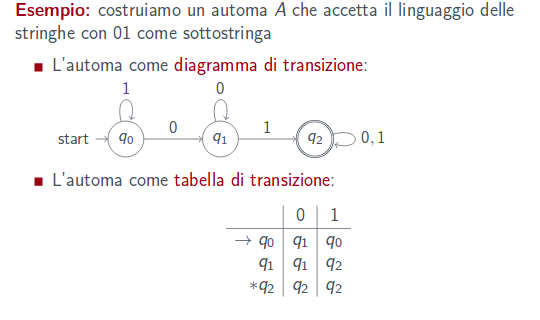
\includegraphics[scale=0.5]{Immagini/DFA.png}
\end{figure}

\section{Linguaggio accettato da un DFA} 
La funzione di transizione prende in input uno stato e una parola dando in output
una nuova parola. Definizione:
\begin{itemize}
\item \textbf{base}: $\delta(q,\varepsilon)=q$ -> ritorna lo stadio in cui è
\item \textbf{induzione} $\widehat{\delta}(q,w)=\delta(\widehat{\delta}(q,x),a)$, 
dove $\widehat{\delta}$ rappresenta lo stato attuale e $\delta$ lo stato in cui mi 
troverò, a indica l'ultima lettera della parola che voglio leggere
NB: in $\delta'$ faccio la ricorsione fino ad arrivare al caso base 
\end{itemize}
Detto ciò, possiamo definire il linguaggio accettato da A in questo modo:
$L(A)=\{w: \widehat{\delta}(q0,w) \in F\}$. Tutti i linguaggi accettati da DFA 
vengono chiamati \textbf{linguaggi regolari}.